\subsection*{Introducción a la teoría de juegos}
La teoría de juegos es una manera de modelar distintos tipos de interacciones de competición, cooperación y otras. Modelar qué decisión y el por qué puede ser tan simple como complejo dependiendo de los factores que que consideremos relevantes. En este capítulo se trataran los juegos simultáneos en secuencia e iterados (también llamados repetidos). 

\section{Juegos simultaneos}

En juegos simultáneos los agentes toman decisiones al mismo tiempo, estas decisiones interactuan resultando en \textbf{pagos}. El pago a cada persona refleja un nivel de utilidad, por lo que cada agente buscará llegar a un resultado del juego (la combinación de acciones) que maximize su pago. 

Para dos agentes $A$ y $B$ cada uno toma la decisión $X$ o $Y$, la combinación de decisiones llevará a cierto nivel de pagos. Este escenario puede ser representado por una \textbf{matriz de pago}\marginnote{\textbf{Matriz de pago:} La matriz de pago es una representación de los pagos un juego simultáneo para un número definido de individuos y estrategias.}[-3cm] en el cuadro \ref{cuadro: matriz de pago genérica}.

\begin{table}[!htbp]
  
  \centering
  \caption{Matriz de pagos}
  \setlength{\extrarowheight}{2pt}
  \label{cuadro: matriz de pago genérica}
  \begin{tabular}{*{4}{c|}}
    \multicolumn{2}{c}{} & \multicolumn{2}{c}{$B$}\\\cline{3-4}
    \multicolumn{1}{c}{} &  & X  & Y \\\cline{2-4}
    \multirow{2}*{$A$}  & X & $(a,b)$ & $(c,d)$ \\\cline{2-4}
    & Y & $(e,f)$ & $(g,h)$ \\\cline{2-4} 
  \end{tabular}
\end{table}

Ejemplifiquemos cómo se lee la tabla. Si $A$ tomó la estrategia $X$ y $B$ toma la decisión $Y$ entonces los pagos correspondientes son $(c,d)$, donde $c$ es el pago para $A$ y $d$ el pago para $B$. De la misma manera si $A$ elije $Y$ y $B$ decide $Y$ la matriz de pagos será $(g,h)$. 

Hay un componente estratégico en la interacción de $A$ y $B$ pues los pagos que reciba cada uno dependerá de la decisión que tome el otro. Por ejemplo si $A$ sabe que $B$ decide $X$ entonces $A$ elegirá la estrategia que maximize sus pagos. Específicamente $A$ está decidiendo con respecto a los pagos en negrita en el cuadro \ref{cuadro: B decide X}.

\begin{table}[!htbp]
  \centering
  \caption{Matriz de pagos con $B$ decidiendo $X$} \label{cuadro: B decide X}
  \setlength{\extrarowheight}{2pt}
  \begin{tabular}{*{4}{c|}}
    \multicolumn{2}{c}{} & \multicolumn{2}{c}{$B$}\\\cline{3-4}
    \multicolumn{1}{c}{} &  & X  & Y \\\cline{2-4}
    \multirow{2}*{$A$}  & X & $(\textbf{a,b})$ & $(c,d)$ \\\cline{2-4}
    & Y & $(\textbf{e,f})$ & $(g,h)$ \\\cline{2-4}  
  \end{tabular}
\end{table}

La decisión que tome $A$ dependerá qué pago es mayor, $a$ ó $e$, si es $a$ entonces elije $X$ y caso contrario elije $Y$.

\subsection{Estrategias y resolución de juegos}

\subsection{Equilibrios de Nash y óptimos de pareto en juegos}

\subsection{Juegos canónicos}

\subsubsection*{Dilema del prisionero}

El dilema del prisionero describe la situación en que dos criminales sospechosos son detenidos y separados para un proceso de interrogación. Si uno de los dos delata al otro y su complice no, este último tendrá pena de cárcel y el delator quedará libre. En caso de que los dos se delaten entre sí, ambos son condenados a años de cárcel. Por útlimo si ninguna se delata entre sí, quedan libres o cumplen penas menores.

La matriz de pago específicamente se en el cuadro. A mayor pena menor es el pago. 

\begin{table}[!htbp]
    \centering
    \caption{El dilema del prisionero}
    \setlength{\extrarowheight}{2pt}
    \begin{tabular}{*{4}{c|}}
      \multicolumn{2}{c}{} & \multicolumn{2}{c}{Prisionero $B$}\\\cline{3-4}
      \multicolumn{1}{c}{} &  & Cooperar  & Delatar \\\cline{2-4}
      \multirow{2}*{Prisionero $A$}  & Cooperar & $(-2,-2)$ & $(-10,-1)$ \\\cline{2-4}
      & Delatar & $(-1,-10)$ & $(-6,-6)$ \\\cline{2-4}
    \end{tabular}
  \end{table}

Cada uno tiene una estrategia dominante en delatar al otro, el resultado es un equilibrio de Nash sub-óptimo en términos de Pareto. 

El juego describe como dos personas no cooperan incluso si ello va en contra del interés de las dos. 

\subsubsection*{Mano invisible}

Si se deja la autorregulación de los mercados, dado que los individuos persiguen su propio interés, se produce un equilibrio que es un óptimo de Pareto. Una matriz que lo representa puede ser.

El agente $A$ tendrá una estrategía dominante, la cual será la opuesto a la del otro agente $B$. Finalmente el equilibrio de Nash es eficiente paretianamente.

\begin{table}[!htbp]
    \centering
    \caption{La mano invisible}
    \setlength{\extrarowheight}{2pt}
    \begin{tabular}{*{4}{c|}}
      \multicolumn{2}{c}{} & \multicolumn{2}{c}{Agente $B$}\\\cline{3-4}
      \multicolumn{1}{c}{} &  & $X$  & $Y$ \\\cline{2-4}
      \multirow{2}*{Agente $A$}  & $X$ & $(0,10)$ & $(1,1)$ \\\cline{2-4}
      & $Y$ & $(11,11)$ & $(10,0)$ \\\cline{2-4}
    \end{tabular}
  \end{table}

%(Aquí se podría citar a Adam Smith)

\subsubsection*{Guerra de los sexos}

Una pareja heterosexual se encuentra incomunicada en medio de un festival de metal. El hombre es fan de Metallica y la mujer fan de Megadeth. 

\begin{table}[!htbp]
    \centering
    \caption{Guerra de los sexos}
    \setlength{\extrarowheight}{2pt}
    \begin{tabular}{*{4}{c|}}
      \multicolumn{2}{c}{} & \multicolumn{2}{c}{Mujer}\\\cline{3-4}
      \multicolumn{1}{c}{} &  & Metallica  & Megadeth \\\cline{2-4}
      \multirow{2}*{Hombre}  & Metallica & $(2,1)$ & $(1,1)$ \\\cline{2-4}
      & Megadeth & $(0,0)$ & $(1,2)$ \\\cline{2-4}
    \end{tabular}
  \end{table}

  Cada uno tiene estragia dominante por ir al concierto de su banda preferida idependiente de lo que haga el otro, hay dos equilibrios de Nash por lo tanto este juego tiene ser resuelto con estrategias mixtas.

\subsubsection*{La caza del venado}
Dos individuos van a cazar ya sea conejos o venados y deben escoger su presa sin conocer la elección del otro cazador. Para cazar el venado (un premio mayor) requieren de la ayuda del otro, mientras que un conejo puede ser cazado por cada uno. Por lo tanto, si cooperan cazando al venado podrán ambos obtener más beneficios y estár en un óptimo de Pareto.

\begin{table}[!htbp]
    \centering
    \caption{La caza del venado}
    \setlength{\extrarowheight}{2pt}
    \begin{tabular}{*{4}{c|}}
      \multicolumn{2}{c}{} & \multicolumn{2}{c}{Cazador $B$}\\\cline{3-4}
      \multicolumn{1}{c}{} &  & Venado  & Conejo \\\cline{2-4}
      \multirow{2}*{Cazador $A$}  & Venado & $(4,4)$ & $(0,3)$ \\\cline{2-4}
      & Conejo & $(3,0)$ & $(3,3)$ \\\cline{2-4}
    \end{tabular}
  \end{table}
En este caso no existen estrategias dominantes, lo que lleva a la existencia de dos equilibrios de Nash, cazar al venado juntos domina paretianamente a cazar conejos juntos. Lo anterior representa un problema de cooperación social y una dicotomía entre seguridad y cooperación. 
\subsubsection*{Chicken}

Se trata de un juego para determinar quien es el más valiente, dos personas se posicionan con sus autos en dos extremos y aceleran de manera que llegará un punto en que choquen entre si. El primero que doble para evitar el impacto es un gallina, dejando al ganador como valiente. Hay tres escenarios, el primero en que uno de los dos dobla y queda como gallina, un segundo escenario en donde los dos doblan ambos quedando como gallinas y por último el caso en que chocan. 

Ambos corredores quieren hacer lo opuesto a lo que haga el otro, los equilibrios de Nash serían entonces los que uno de ellos dobla y el otro sigue. Lo cual puede expresarse por medio de la matriz de pago.\footnote{Rising, L: The Patterns Handbook: Techniques, Strategies, and Applications, page 169. Cambridge University Press, 1998. \textbf{Schedule Chicken}.}
\begin{table}[!htbp]
    \centering 
    \caption{Chicken}
    \setlength{\extrarowheight}{2pt}
    \begin{tabular}{*{4}{c|}}
      \multicolumn{2}{c}{} & \multicolumn{2}{c}{Corredor $B$}\\\cline{3-4}
      \multicolumn{1}{c}{} &  & Ceder (gallina)  & Seguir (valiente) \\\cline{2-4}
      \multirow{2}*{Corredor $A$}  & Ceder (gallina) & $(2,2)$ & $(1,3)$ \\\cline{2-4}
      & Seguir (valiente) & $(3,1)$ & $(0,0)$ \\\cline{2-4}
    \end{tabular}
  \end{table}

\section{Juegos secuenciales}

Los juegos secuenciales son una forma extendida de lo que se ha aplicado hasta ahora. Antes las estrategias eran acciones individuales; confesar, delatar, cooperar, tracionar, etcéra, ahora serán planes completos de acciones. 

Lo ejemplos más usados son respecto al uso de bombas nucleares durante la guerra fría, también aprovechemos recordar como se planteaban estos juegos. Nuestro juego parte de una situación en que la Unión Soviética exige a las potencias
occidentales que abandonen Berlín. En este punto, Estados Unidos tiene dos posibilidades:
Aceptar y No aceptar.

\begin{center}
    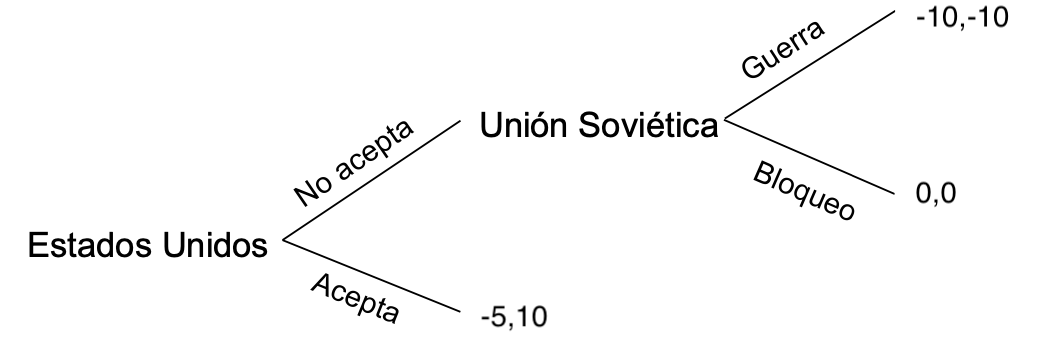
\includegraphics[scale=0.5]{Figuras/juegos secuencia.png}  
\end{center}
Las estrategias serán un plan de acción, en esta caso serían (Acepta, No Acepta y Guerra, No Acepta y Bloqueo).

Para resolver estos juegos uno tiene que seguir un método inductivo, resolver desde el futuro hacia el pasado. ¿Por qué resolver de adelante hacia atrás? Porque si resolvieramos como en juegos simultáneos no estaríamos contando si la amenaza (en este caso una respuesta bélica) es creíble. 

Si plantearamos de manera simultánea encontramos dos EN, uno (el de Acepta y Guerra) en que \textbf{no es secuencialmente racional}, para que ese equilibrio sea posible Estados Unidos tiene que aceptar, sin embargo veremos a continuación por qué si Estados Unidos no acepta la Unión Soviética nunca responderá con una respuesta bélica.

\begin{table}[!htbp]
    \centering
    \caption{Dominio sobre Berlín}
    \setlength{\extrarowheight}{2pt}
    \begin{tabular}{*{4}{c|}}
      \multicolumn{2}{c}{} & \multicolumn{2}{c}{Unión Soviética}\\\cline{3-4}
      \multicolumn{1}{c}{} &  & Guerra & Bloqueo \\\cline{2-4}
      \multirow{2}*{Estados Unidos}  & Acepta & $(\underbar{-5},\underbar{10})$ & $(-5,10)$ \\\cline{2-4}
      & No acepta & $(-10,-10)$ & $(\underbar{0},\underbar{0})$ \\\cline{2-4}
    \end{tabular}
  \end{table}

El juego tiene que ser \textbf{secuencialmente racional} por lo que resolvemos de adelante hacia atrás. El resultado será un equilibrio perfecto en subjuegos (EPS).

Por lo tanto primero se resuelve la decisión de la Unión Soviética, la cual debiese decidir bloquear, y luego evaluar que decidirá Estados Unidos, la cual debiese no aceptar. 

\begin{center}
    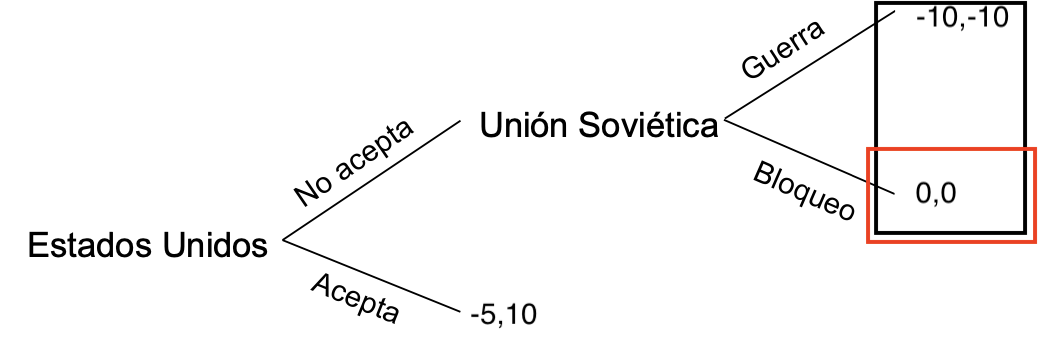
\includegraphics[scale = 0.50]{Figuras/Inducción.png}
\end{center}

\subsubsection*{Relación EN y EPS}

En un juegos secuencial puedes obtener EN que no sean coherentes con las amenazas creíbles. Los EPS siempre son coherentes con la credibilidad de las amenazas. \textbf{Un EN no siempre es un EPS, pero un EPS siempre es un EN}. 